\documentclass[a4paper,10pt]{article}
%A Few Useful Packages
\usepackage{marvosym}
\usepackage{fontspec,enumitem} 					%for loading fonts
\usepackage{xunicode,xltxtra,hyperref,parskip} 	%other packages for formatting
\usepackage[margin=2.5cm]{geometry}
\RequirePackage{color,graphicx}
\usepackage[usenames,dvipsnames]{xcolor}
\usepackage[big]{layaureo} 				%better formatting of the A4 page
% an alternative to Layaureo can be ** \usepackage{fullpage} **
\usepackage{array,xeCJK}
\usepackage{titlesec}					%custom \section
\setlist[itemize]{leftmargin=0pt}

%Setup hyperref package, and colours for links
\usepackage{hyperref}
\definecolor{linkcolour}{rgb}{0,0.2,0.6}
\hypersetup{colorlinks,breaklinks,urlcolor=linkcolour, linkcolor=linkcolour}

%FONTS
\defaultfontfeatures{Mapping=tex-text}
\newfontface\TitleFont{Noto Sans}
\setmainfont{Noto Sans}
\setsansfont{Noto Sans}
\setCJKmainfont{Source Han Sans TW}

\titleformat{\section}{\large\bfseries\TitleFont\raggedright}{}{0em}{}[\titlerule]
\titlespacing{\section}{0pt}{1em}{0.5em}

\setlength{\parindent}{0pt}
\newcommand{\leftcolumn}{0.6\textwidth}
\newcommand{\wideleftcolumn}{0.75\textwidth}
\newcolumntype{L}{>{\raggedright\arraybackslash}p{\leftcolumn}}
\newcolumntype{W}{>{\raggedright\arraybackslash}p{\wideleftcolumn}}
\newcommand{\rightcolumn}{\textwidth-\leftcolumn-1cm}
\newcommand{\narrowrightcolumn}{\textwidth-\wideleftcolumn-1cm}
\newcolumntype{R}{>{\raggedleft\arraybackslash}p{\rightcolumn}}
\newcolumntype{X}{>{\raggedleft\arraybackslash}p{\narrowrightcolumn}}
\newcommand{\tablespacer}{\multicolumn{2}{c}{}\\}
\newcommand{\entry}[1]{\textsf{#1}}
\newcommand{\md}{$\cdot$ }
\newenvironment{cvtable}{\begin{tabular}{WX}}{\end{tabular}}
\newenvironment{cvtable*}{\begin{tabular}{LR}}{\end{tabular}}

\usepackage{multicol}
\begin{document}
\pagestyle{empty} % non-numbered pages
\frenchspacing

% Title

\begin{center}
  \Huge{Hu Shuhan 
\includegraphics[height=1.2em,trim=0 10mm 0 -1cm]{shared/signature.png}}\par

\normalsize 245, Section 5, Roosevelt Road, Wenshan District, Taipei City 116, Taiwan 
\vspace*{.3em}

  
\includegraphics[width=0.5em]{shared/mobile-alt.eps} {+886 910-384-478} $\cdot$
  
\includegraphics[width=0.8em]{shared/envelope.eps} {1119han@gmail.com} $\cdot$
  
\includegraphics[width=0.8em]{shared/github.eps}
  \href{https://github.com/RocketSH}{github.com/RocketSH} 

\rule{15.2cm}{0.05em}
\vspace*{.5em}
\begin{center}
  \large{\textbf{Objective: Frontend Developer}}
\end{center}
\vspace*{.5em}

\begin{center}
  \begin{minipage}{0.9\textwidth}
    Four years in footwear manufacturing made me understand that although automation techniques are already commonly
    implemented on the factory floor, there are still many repetitive, everyday tasks in office work that remain to be optimized. Therefore I have decided to learn software development to be able to \textbf{automate} day-to-day tasks and \textbf{save
    time and money}, both for my clients and for myself.
    \vspace*{1em}\\
    I have recently graduated from a three-month bootcamp organized by 5xRuby, a Taiwan-based
    software development company specializing in Ruby on Rails.
    During the course, I have learned the basics of \textbf{HTML, CSS, Bootstrap, Ruby on
    Rails, JavaScript and Git version control}, also self-learned
    \textbf{PostgreSQL, ReactJS}.
  \end{minipage}
\end{center}
\vspace*{.8em}

\begin{center}
  \large{\textbf{Profolio}}
\end{center}
\vspace*{.3em}

\begin{minipage}{1\textwidth}
\hspace*{1em}\entry{Personal Blog}

\includegraphics[width=0.8em, center]{shared/globe-asia.eps}
\href{https://rocketgirl.io/}{rocketgirl.io}

\hspace*{1.5em}{ReactJS, HTML, CSS, GatsbyJS}
\end{minipage}
\begin{minipage}{0.5\textwidth}
  \hspace*{1em}\entry{Email Newsletter Website}
  
\includegraphics[width=1em]{shared/mail.png}
  \href{https://www.goodbyt.es/}{goodbyt.es}

  \vspace*{.5em}
  \hspace*{1.5em}{[Frontend] HTML, CSS, Bootstrap, SortableJS, AJAX}
  \hspace*{1.5em}{Stimulus}
  
  \vspace*{.5em}
  \hspace*{1.5em}{[Backend] Ruby on Rails} 

  \vspace*{.5em}
  \hspace*{1.5em}{[Ruby Gem] Devise, Nokogiri, Carrierwave, AWS S3}

  \vspace*{.5em}
  \hspace*{1.5em}{[Database] PostgreSQL} 

  \vspace*{.5em}
  \hspace*{1.5em}{[Email Service Provider] Mailgun}
  \vspace*{1em}

\end{minipage}%
\begin{minipage}{0.5\textwidth}
  \vspace*{.8em}
  \begin{center}
    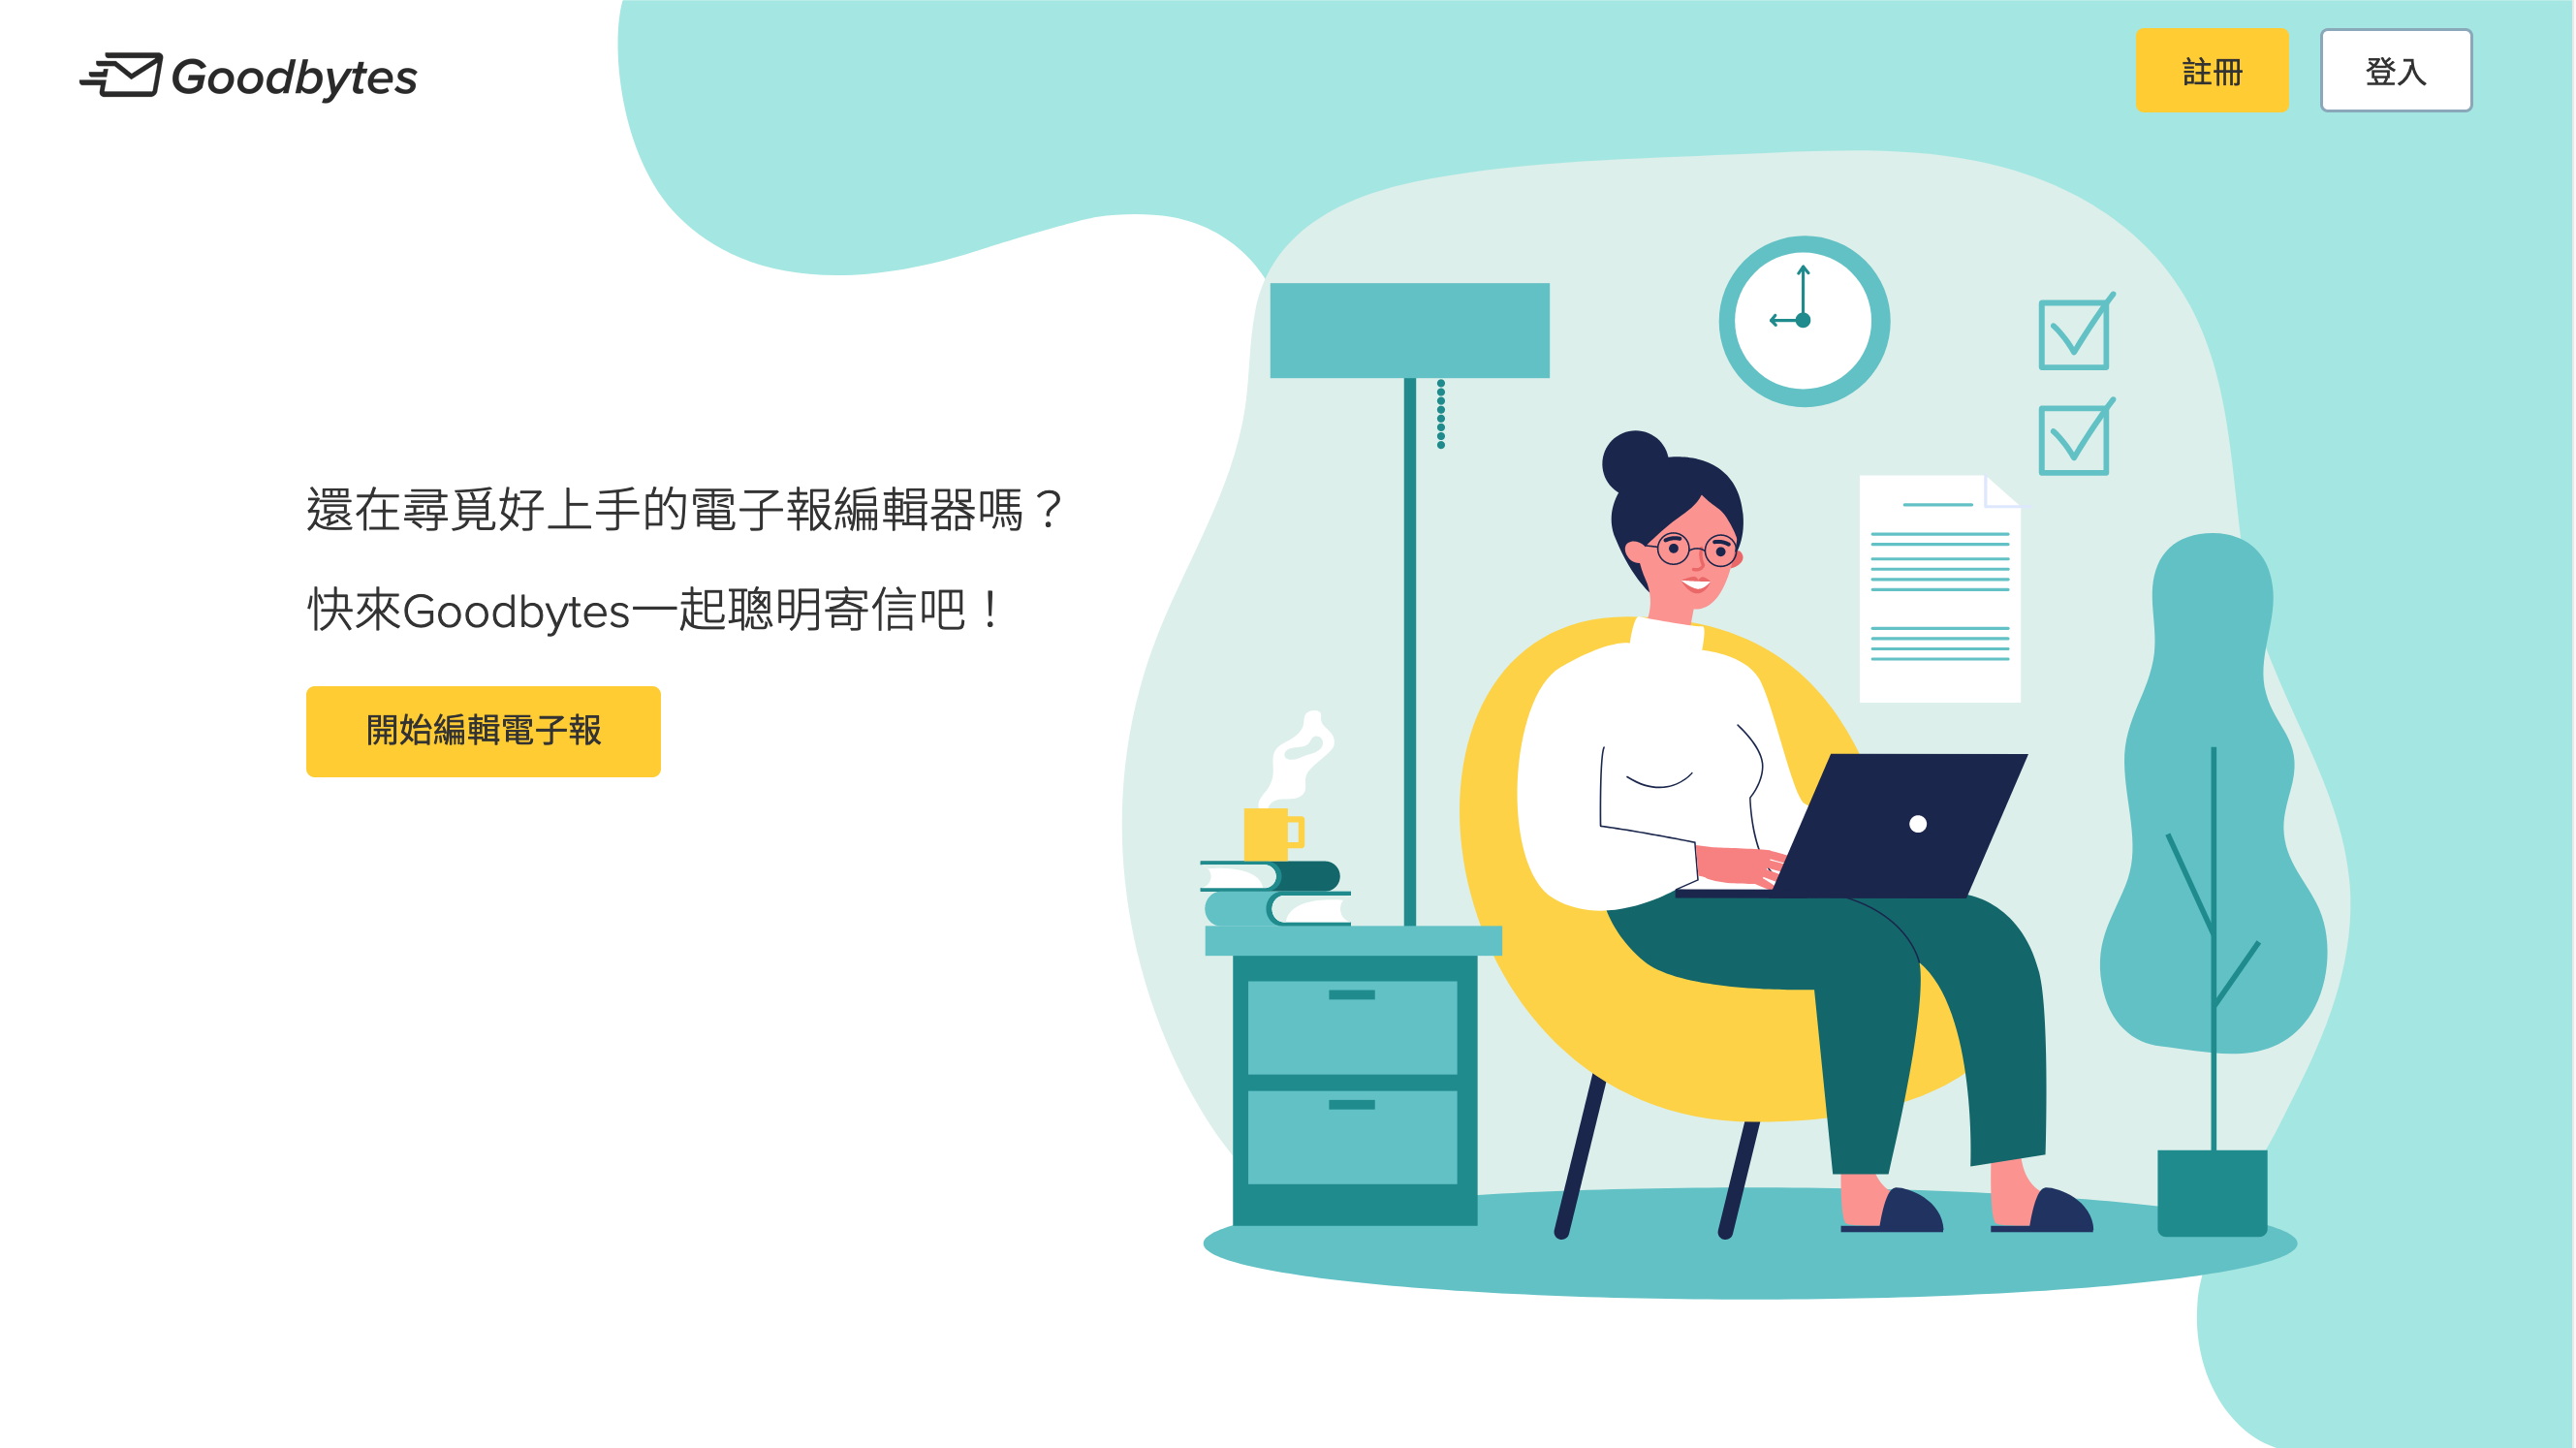
\includegraphics[width=7cm]{shared/landing.png}
  \end{center}
\end{minipage}

\section{Work Experience}
\setlength{\leftskip}{1em} 
\begin{cvtable*}

  \hspace*{-1em}\entry{Pouchen Group} & Jul 2015--Oct 2019 \\[.9em]

  \entry{SAP CO of Data Conversion Specialist, Pouchen Group} & Taichung, Taiwan \\
  \begin{itemize}
      \item Assisted the migration of footwear-related data from a legacy ERP
        system within six-month
      \item Set up \textbf{data transformation logic}, \textbf{testing and debugging of data extraction procedures}, \textbf{analyzing error logs}
  \end{itemize}
  & Jun 2019--Oct 2019 \\

  \entry{Footwear Costing Supervisor, Pouchen Group} & Ho Chi Minh City, Vietnam \\
  \begin{itemize}
      \item Cooperated with the brand leadership of Salomon, Arc'teryx, Mavic, and Wilson, as well as the Development and Merchandising departments in order to optimize costs based on the target FOB
      \item Assisted subordinate ten Taiwanese and Vietnamese team members with Cost Breakdown analysis
  \end{itemize} & May 2017--Jun 2019 \\

  \entry{Footwear Costing Specialist, Pouchen Group} & Dongguan, China \\
  \begin{itemize}
  \item Collecting raw material price and negotiating product specifics with Tier Two suppliers twice a year
  \item Collecting and analyzing product-related tasks assigned by the Product
    Manager and Costing Manager twice a year for business negotiation with client
  \end{itemize}  & Jul 2015--May 2017 \\
\end{cvtable*}

\begin{cvtable*}
  \entry{Credit Card Specialist, Citibank} & Taipei, Taiwan \\
  \begin{itemize}
  \item Application verification
    \end{itemize} & Jul 2013--Nov 2014 \\
  \setlength{\leftskip}{0pt} 
\end{cvtable*}

\section{Education}

\begin{cvtable*}

  \entry{\textsc{Astro Camp} Ruby on Rails Bootcamp, 5xRuby} & Taipei, Taiwan \\
  Ruby, Ruby on Rails, HTML, CSS, and ES6 & March--June 2020 \\
  \tablespacer

  \entry{National Dong Hwa University, College of
Management} & Hualien, Taiwan \\
  Bachelor of Arts --- Double Major in Economics and Business Administration in Finance & Graduated June 2013 \\
  \tablespacer

\end{cvtable*}

\section{Other Skills}
\begin{cvtable*}
  \begin{itemize}
    \item{Chinese (Mandarin)} --- Native Language, {English} --- Fluent (TOEIC 840), {Vietnamese} --- Basic (A2)
    \item Microsoft Excel PivotTable report, Google Docs, iWork
  \end{itemize}
\end{cvtable*}
\end{document}
